\chapter{Wearable Cognitive Assistance Development Tools}
\label{chapter: app-dev}

While previous chapters address the system challenges of scaling wearable
cognitive assistance at the edge, another key obstacle to the widespread
adoption of WCAs is the level of specialized skills and the long development
time needed to create new applications. Such expertise include task domain
knowledge, networked application development skills, and computer vision
insights. Researchers~\cite{chen2018application} report that it typically takes
multiple person-months of effort to create a single application. The majority of
development time is spent on learning new computer vision techniques, selecting
robust algorithms to use through trial and error, and implementing the
application. The high barrier of entry significantly limit the number of
wearable cognitive assistants available today. Clearly, this is not scalable. 

In this chapter, we reflect on existing ad hoc WCA development process, propose
a new development methodology centered around DNN-based object detection, and
present development tools we have built to lower the barrier of WCA development.
Our goal is to simplify the process so that a small team (1-2 people) of a task
expert and a developer, without computer vision expertise, can create an initial
version of a Gabriel application within a few days. This is a productivity
improvement of at least one order of magnitude. Refinement and tuning may take
longer, but can be guided by the early use of the application. 

Simplification is difficult. The application needs a precise definition of the
end-point state of each step (e.g., a particular screw mounted into a
workpiece), yet needs to be tolerant of alternative paths to reaching that end
point (e.g., hand-tightening versus using a screwdriver). We assume the small
development team has knowledge of the task specifics and general programming
skills, but not necessarily experiences with wearable devices or computer
vision.

\section{Ad Hoc WCA Development Process}
\label{sec: app-dev-adhoc}

\begin{figure}
  \centering
  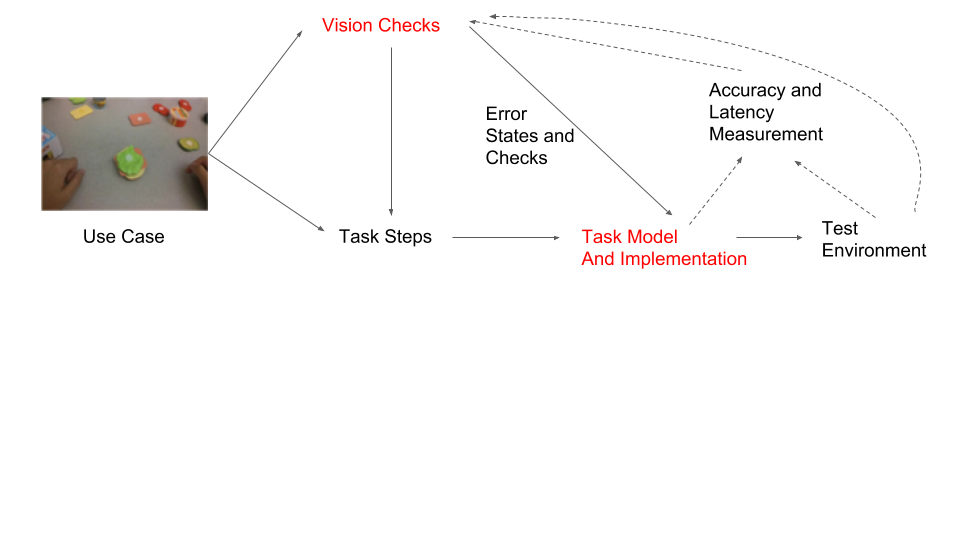
\includegraphics[trim={0 6cm 0 0},width=\linewidth]{FIGS/ad-hoc-workflow}
	\caption{Ad Hoc Development Workflow}
    \label{figs:workflow}
\end{figure}

Existing ad hoc development process of WCAs can be described as
figure~\ref{figs:workflow}. Developers first work with task expert to identify
and pinpoint a specific use case. With the use case in mind, the development
team needs to identify critical visual features and states that can be reliably
recognized with machine vision. In the meantime, the use case is broken down
into individual steps. For each step, feedback messages to users are created
based on detected visual states. Potential errors are also enumerated and
included as additional steps. We refer to the complete set of the steps
annotated with visual states and feedback as the \textit{Task Model}. For
example, for the LEGO wearable cognitive assistance~\cite{chen2017empirical},
the task model contains the sequence of blocks to build up the final assembled
Lego piece, together with potentially misused blocks. The visual states to
recognize are the pieces currently on the lego board: the shape and the color of
individual lego block, and their composed shape and color.

Notably, a task model is not only determined by the task itself, but also
influenced heavily by visual states that can be reliably detected. In fact, it
is common to alter the sequence of steps or introduce additional steps to reduce
the difficulties and improve the reliability of computer vision recognition.
Since there is a human in the loop (the user), relying on humans to do what they
are good at is the main reason that wearable cognitive assistance can be
implemented without solving the generic perception and planning problems
intrinsic to robotics. For example, a frequently used technique is to ask the
user to hold the object of interests at a fixed viewpoint shown in the image
guidance. Narrowing the viewing angle makes the recognition problem more
tractable.

Application task model serves as a blueprint for implementation. For each step
in the task model, developers select and implement computer vision algorithms.
Custom logic is also written to handle step transitions and interface with the
Gabriel platform. After initial implementation, test runs are conducted to
evaluate the robustness of computer vision and measure the end-to-end
application latency. The implementation process is typically iterative to allow
trials and errors when choosing computer vision algorithms.

The ad hoc development process has unnecessary high requirements and burden for
WCA creators in the following aspects.
\begin{enumerate}
  \item Developers need to be familiar with various computer vision algorithms
to determine what visual states can be recognized reliably. The knowledge of
selecting algorithms for specific objects, environments, and setups requires
years of experience. This high bar of entry hinders more WCAs to be developed.
  \item It takes a significant amount of time to implement computer vision
algorithms in a trial and error fashion. Several months of coding time could
turn into a fruitless outcome when the algorithm turns out to be a bad fit. For
sophisticated WCAs with tens or hundreds of visual states, such a trial and
error methodology is not scalable. Needed are unified and automated methods to
create visual state recognizers.
  \item The tight coupling of task model design and visual state recognition
calls for deep understanding in both task domain and computer vision. When
visual states in the task model end up being too difficult for even the
state-of-art algorithms, the development team needs to adjust the task model to
either use alternative visual states or employ user assistance. For instance, in
the RibLoc application, during development, a task step was changed to asking
the user to read out a word on the gauge instead of performing optical character
recognition on the lightly-colored characters. Close collaborations among task
experts and developers are needed due to this tight intertwinement between task
model design and computer vision algorithm exploration. Methodologies and tools
that shorten the turn-around time when a task model changes can significantly
reduce the overall development time.
\end{enumerate}


% Among all the development procedures, creating the computer vision checks to
% detect user states consumes the most of development time and requires computer
% vision expertise and experience. With the adoption of DNNs, developers no longer
% need to spend days to select and tweak handcrafted features. Instead, the entire
% model is trained end-to-end using labeled data. However, DNNs, with millions of
% parameters to train, requires a significant amount of training data. Collecting
% and labeling data are time-consuming and painstaking. Besides, to craft and
% implement a DNN by hand is not trivial. Significant machine learning background
% is needed to tweak network architectures and parameters. Therefore, developer
% tools are needed to both help label the data and create deep neural networks.

% In summary, implementing the workflow of cognitive assistance takes time and
% efforts. Ad-hoc implementation requires a team of domain experts, developers and
% computer vision experts. Such development model cannot scale to thousands of
% applications. Therefore, Gabriel needs to be extended with tools to reduce the
% effort of creating wearable cognitive assistants.

% Existing ad-hoc approach to develop wearable cognitive assistance not only takes
% a long time, but also requires significant amount of computer vision expertise.
% Developers new to wearable cognitive assistance would need to spend months
% learning computer vision basics and acquire intuitions to determine what is
% achievable before developing an application. 

% Figure~\ref{fig:workflow} shows the ad-hoc development process. 

\section{A Fast Prototyping Methodology}

To streamline the development process and lower the barrier of entry, we propose
a new prototype methodology which focuses on the following two aspects.
\begin{enumerate}
  \item  Use deep neural network (DNN) based object detection as the universal
  building block for visual state recognition.
  \item Use finite state machine to represent and implement application task model.
\end{enumerate}
We first introduce the concepts of this methodology and describe its benefits in
this section and then introduce tools we have built to automate the development
process in subsequent sections.

\subsection{Objects as the Universal Building Blocks}

To replace manual selection of computer vision algorithms through trial and
error, we propose to use DNN-based object detection as the fundamental building
block to detect user states. Using object detection as the universal building
block means that each visual state should be decomposed and described as a
collection of individual objects along with their attributes and relationships.
We argue that objects as fundamental building blocks provide expressive and
flexible constructions capable of describing a wide range of visual user states
important to WCAs. Intuitively, the addition and removal of objects from a scene
is straightforward to express. Spatial relationships among objects (e.g. close
to, on the left of, overlap significantly) capture semantic visual features that
can be used to infer user states. For example, the detection of two Ikea
furniture pieces close to each other could indicate that they have been
assembled together. Moreover, temporal relationships can add confidence to the
inference made from spatial relationship. The detection of two pieces of
furniture closely connected to each other in the last 30 frames implies strongly
that they have been assembled together. Of course, there are limitations on how
reliable the inference could be. Nonetheless, objects together with their
spatial and temporal relationships with one another, provide a flexible
reasoning framework to decompose user states into visual states.

\begin{figure}
  \centering
  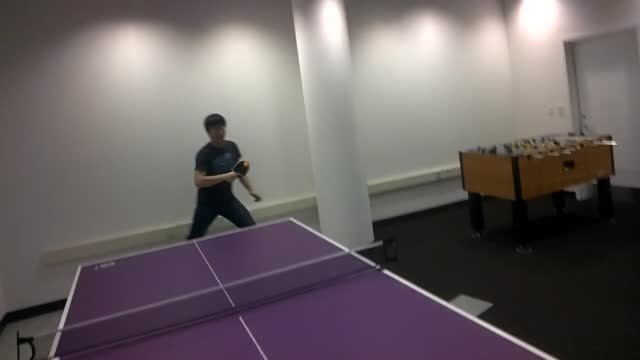
\includegraphics[trim={0 0 0 0},width=.9\linewidth]{FIGS/pingpong}
	\caption{A Frame Seen by the PING PONG Assistance}
    \label{figs:pingpong-frame}
\end{figure}

To illustrate the effectiveness of this object centered approach, we showcase
how existing applications built without this methodology in mind can be easily
expressed. Figure~\ref{figs:pingpong-frame} shows an image that will trigger the
PING PONG assistance to provide an instruction to hit the ball to the left. We
can express this visual state with a collection of objects, namely the Ping-Pong
table, the ball, and the opponent. These objects should satisfy the following
spatial relationship for the instruction ``hit to the LEFT'' to be generated. To
improve the accuracy of our instruction, we can require the spatial relationship
of these objects to be held true for at least two consecutive frames before an
instruction is produced.

\begin{itemize}
  \item The Ping-Pong ball is above the Ping-Pong table for an active rally.
  \item The opponent is on the right side of the Ping-Pong table.
  \item The ball is also on the right side of the Ping-Pong table.
\end{itemize}

\begin{figure}
  \centering
  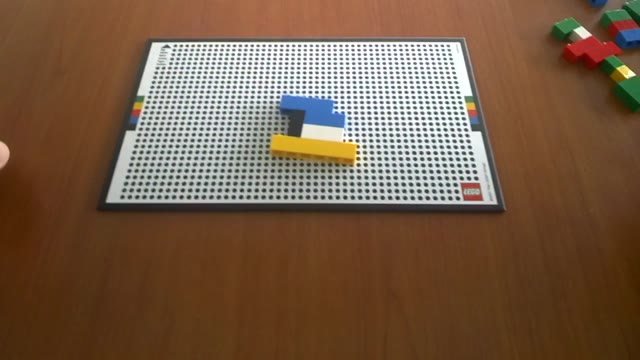
\includegraphics[trim={0 0 0 0},width=.9\linewidth]{FIGS/lego}
	\caption{A Frame Seen by the LEGO Assistance}
    \label{fig:lego-image}
\end{figure}

Similarly, we can express the user states using objects for another
application LEGO. Figure~\ref{fig:lego-image} shows a visual state for the
assembled pieces. Here the collection of objects needs to be present are two
blue Lego blocks, two black blocks, one white block, and one yellow block. The
spatial relationships among these block include:

\begin{itemize}
  \item The yellow block should be at the bottom and longer than all other blocks.
  \item The white block should be in the middle of a blue block and the yellow
  block. It should have the same width as the blue block.
  \item Two black blocks should be on the left of a blue block and the white
  block. It should also be on the bottom of a blue block.
  \item One blue bock should be at the top of all other pieces.
\end{itemize}

One challenge with object detection is to obtain the absolute scale. In this
example, it would be difficult to get the exact width of the lego block (e.g.
whether it is a 1x4 or 1x3 lego piece) with object detection alone. However,
once the location of object is detected, additional processing can be used to
identify object attributes. For example, we can leverage the dots
on the lego board to calculate the absolute size of lego pieces.

The key benefit of using object detection as the universal unit to recognize
visual states is the possibility of automation. In recent years, deep neural
networks have dramatically increased the accuracy of object
detection~\cite{zou2019object}. In 2008, the best object detector, based on
deformable part model~\cite{felzenszwalb2008discriminatively}, achieved a mean
average precision (mAP) of 21\% on the Pascal Visual Object Classes
dataset~\cite{everingham2010pascal}. In less than ten years, deep neural
networks~\cite{he2017mask,Ren2015,He2016,lin2017focal} have quadrupled the
accuracy to 84\% on the same dataset. For a wide range of real-world objects,
DNNs have shown to be effective in both accurate identification of classes and
localization of object bounding boxes.  They can even differentiate subtly
different classes, such as breeds of dogs. Many commercial products now offer
features using DNN object detection. For example, Google
Photos~\cite{googlePhoto} and Pinterest Visual Search~\cite{pinterest} allow
users to search for images containing object of interest using text.

In addition to significant improvement in accuracy, DNNs also provide a unified
method to create object detectors. Modern DNN-based object detection employs an
end-to-end learning approach, in which one or multiple deep neural networks are
trained to predict the object classes and locations directly from RGB images.
Gone is the need of hand-crafted feature engineering. Instead, DNNs, on their
own, find distinguishable features during the training process as they are
presented with labeled examples of different objects. The substitute of custom
CV with machine-learned models makes automation possible. A typical DNN training
process consists of the following steps.

\begin{enumerate}
  \item Collect images of object of interests from diverse background,
  perspectives, and lighting conditions.
  \item Annotate these images with bounding boxes and class names to create a
  dataset of training data, evaluation data, and test data.
  \item Implement a DNN-based object detection network, typically using machine learning frameworks,
  such as Tensorflow~\cite{abadi2016tensorflow} and
  PyTorch~\cite{paszke2019pytorch}.
  \item Continuously train and evaluate a DNN model using the labeled dataset.
  \item Test the accuracy of the trained DNN model on the test data.
\end{enumerate}

While a unified training method eliminates manual feature engineering, creating
a DNN-based object detector is still both time-consuming and painstaking for the
following reasons. First, DNNs often have millions of model parameters and
therefore requires millions of labeled examples to train from scratch.
Collecting and labeling such large amount of training data takes significant
manual labor. Second, implementing a DNN correctly for object detection is not
trivial and still requires significant amount of knowledge of machine learning.
For example, state-of-art object detectors uses custom layers different from the
standard convolutional layer for better performance. Data augmentation, batch
normalization, and drop out are needed at training time for better results
through optimization, but should be disabled during inference time. To
streamline the process of creating DNN-based object detectors, we provide a web
application TPOD (Section~\ref{sec: app-dev-tpod}) that hides the implementation
details from the developers and allow them to train a DNN object detector from a
web browser without writing a single line of code.

\subsection{Finite State Machine (FSM) as Application Representation}
\label{sec: app-dev-fsm-representation}

While the Gabriel platform handles data acquisition and transmission from mobile
wearable devices to cloudlet, application developers still need to write custom
business logic for their own use cases. Since the task model can change
frequently during development, a fast turn-around time to implement changes can
reduce the overall development time. Therefore, we propose a finite state
machine representation of application logic and a GUI tool to enable fast
turn-around. 

Our choice of finite state machine representation is based on the observation
that WCAs, in their nature, consist of states. A FSM ``State'' corresponds to a
user state at a particular time instance. At a given state, the WCA runs
computer vision processing specific to the state to analyze the current scene.
We refer to the computer vision algorithms as ``Processors'' for the state. The
outputs of ``Processors'' are symbolic states of current scene. For example, a
symbolic state can be a vector of objects. ``Transitions'' to other states
happen when the symbolic states meet some criteria, for example, the presence of
a new object. We refer to these criteria as ``Predicates'' for transitions. A
``State'' can have multiple transitions into different adjacent ``States''. Each
``Transition'' has its own ``Predicate''. ``Transitions'' also have the concept
of precedence. The first ``Transition'' whose ``Predicate'' is satisfied is
triggered for a state change. In addition to predicates, ``Transitions'' also
have guidance instructions. When a ``Transition'' is taken, the corresponding
guidance instruction is delivered to the user.


\begin{figure}
  \centering
  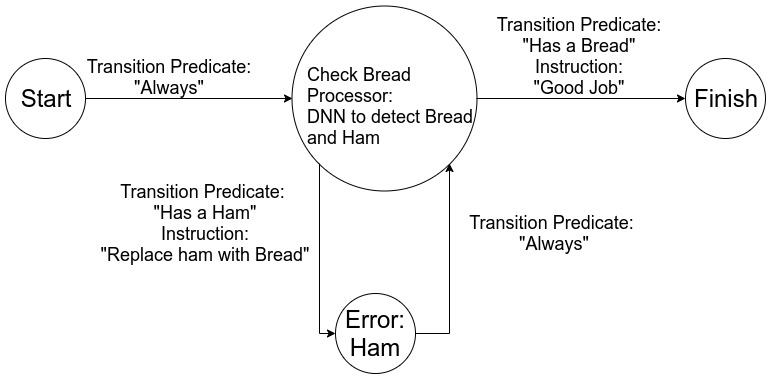
\includegraphics[trim={0 0 0 0},width=\linewidth]{FIGS/fsm-example}
	\caption{Example WCA FSM}
    \label{figs:fsm-example}
\end{figure}

Figure~\ref{figs:fsm-example} shows an example of a simple WCA represented as a
finite state machine. This example WCA checks whether a piece of bread is
present. If so, it congratulates the user. On the other hand, if it detects a
piece of ham is present, a corrective guidance is sent to the user. There are
four states in total. The application starts from the ``Start'' state and
immediately transitions to ``Check Bread'' state as the predicate is ``Always''.
At ``Check Bread'' state, for each frame, a DNN to detect bread and ham is run
to extract the symbolic state. Then, every transition is checked to see if its
predicate is satisfied. If a ``Bread'' is detected, the transition predicate to
the ``Finish'' state is satisfied and hence the transition taken. The
corresponding instruction ``Good Job'' is delivered to the user. Similarly, when
in ``Check Bread'' state, if a ``Ham'' is detected, the transition to the
``Error: Ham'' state is satisfied and taken. The instruction ``Replace Ham with
Bread'' would be delivered as the corrective guidance to the user.

With an FSM representing custom application logic, we impose structure on the
the WCA application. We provide a python API and a web GUI, introduced in
Section~\ref{sec: app-dev-fsm}, to enable developers to quickly create a
FSM-based cognitive assistant. 

\section{Tools For Painless Object Detection (TPOD)}
\label{sec: app-dev-tpod}

Training a DNN for object detection is not trivial.  In particular, it involves
constructing a correctly-labeled training data set with millions of positive and
negative examples. The training process itself may take days to complete, and
involves a set of arcane procedures to ensure both convergence and efficacy of
the model. Fortunately, one does not typically need to train a DNN from scratch.
Rather, one can start with a pretrained model based on a public image data set
such as ImageNet, and then adapt it to detect custom classes for a new
application, though a process called \emph{transfer learning}.  The key idea is
that much of the training teaches the model to discover low-level features, such
as edges, textures, shapes, and patterns that are useful in distinguishing
objects, and such features can largely be reused in other detection tasks on
similar images.  Thus, adapting a pretrained model for new object classes
requires only thousands of examples and hours of training time. 

However, even with transfer learning, collecting a labeled training set of a
thousand examples per object class can be a daunting and painful task. In
addition, implementing DNNs requires expertise and takes time. TPOD is a
web-based tool we developed to streamline the process of creating DNN-based
object detectors for fast prototype. It provides a tracking-assisted labeling
interface for speedy annotation and transfer learning-based DNN training and
evaluation backends that abstract the nuances of DNNs. It helps to greatly
reduce the labeling effort while constructing the dataset, and automates and
takes some of the guesswork out of training a DNN model.

% A user would first
% upload short videos of the object collected from varying lighting conditions and
% perspectives. Then, the user would label these objects using TPOD's labeling
% interface. TPOD assists labeling by tracking the labeled object across frames.
% Augmenting training data with synthetically generated data is also supported. A
% user then can start training from the web interface. TPOD backend uses transfer
% learning to finetune an object detector DNN from publicly available networks
% that have been trained with millions of images. When the training is done, a
% user can downl.oad the object detector as a container image to run the trained
% models for inference. TPOD also provides interfaces for evaluating and testing
% trained DNNs.

\subsection{Creating a Object Detector with TPOD}

\begin{figure}[]
  \centering
  \begin{minipage}[b]{0.32\textwidth}
    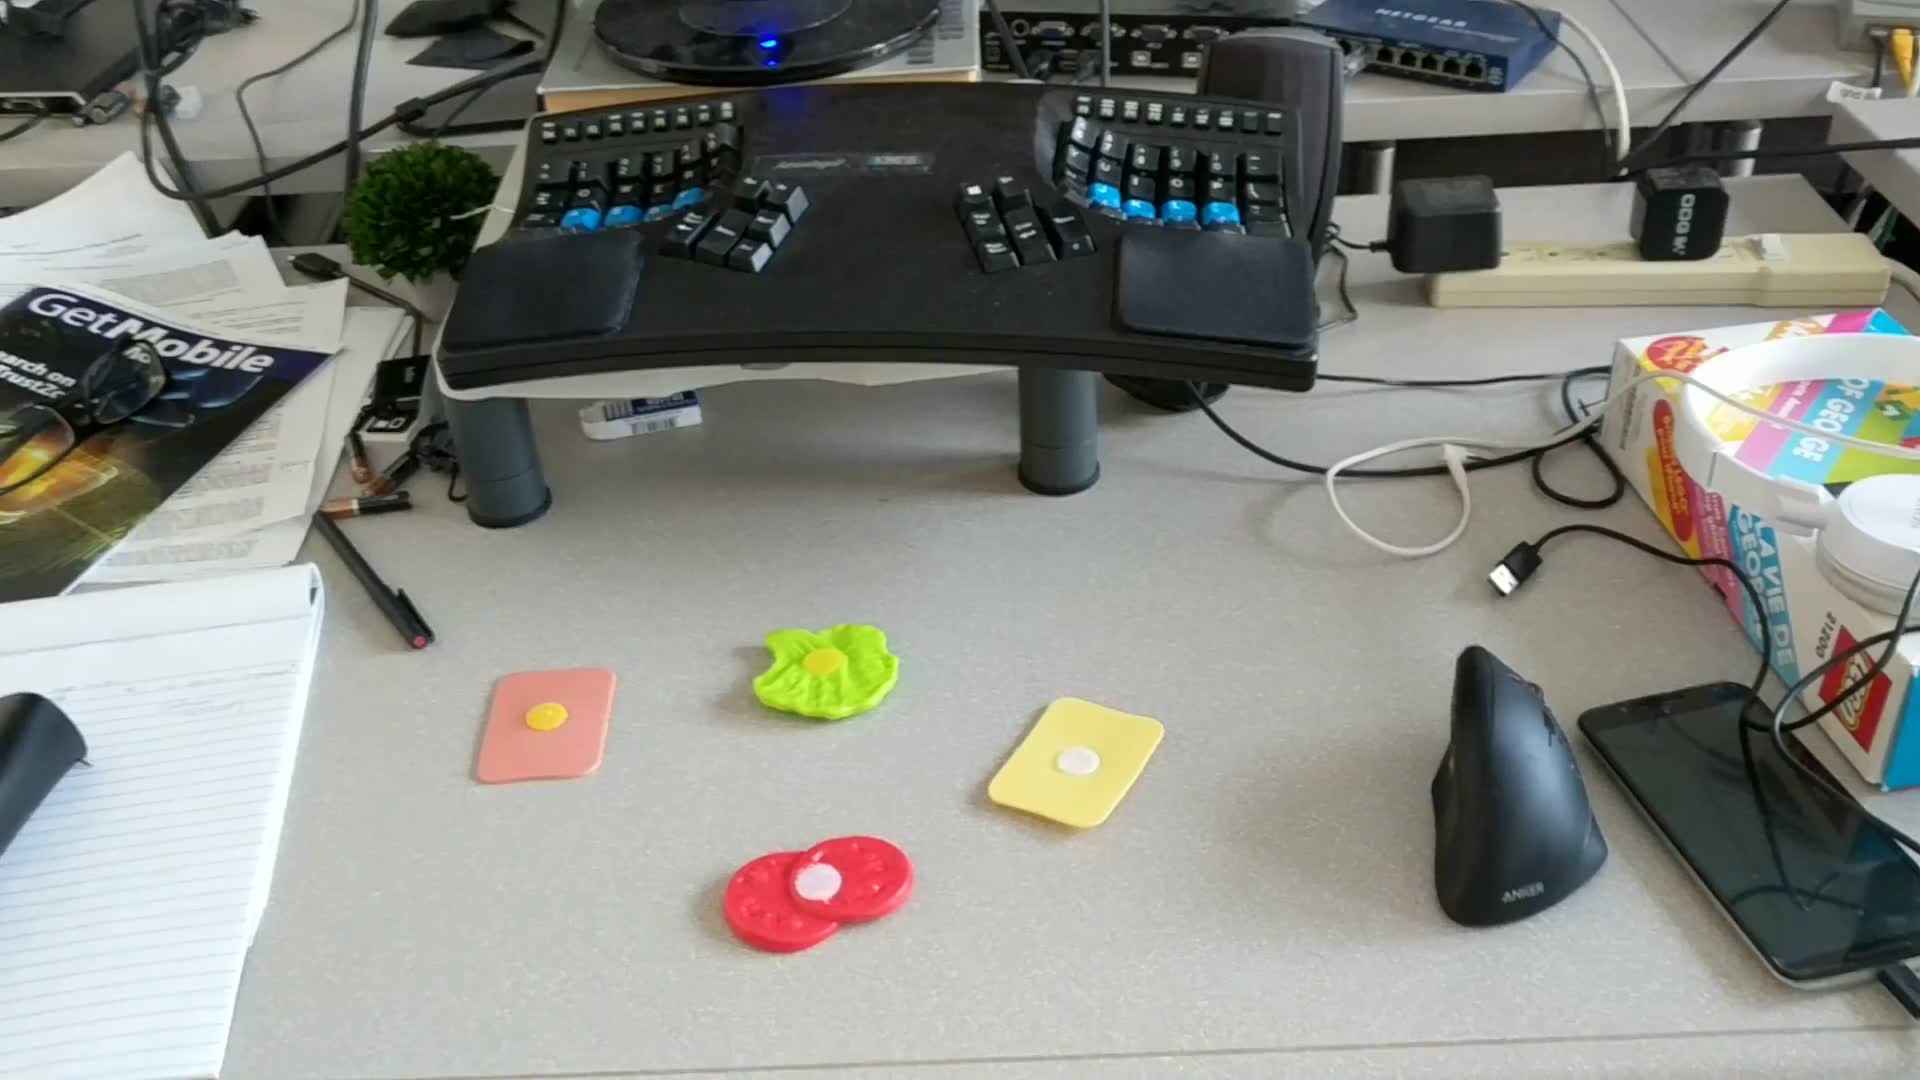
\includegraphics[width=\textwidth]{FIGS/sandwich-training-1.jpg}
  \end{minipage}
  \begin{minipage}[b]{0.32\textwidth}
    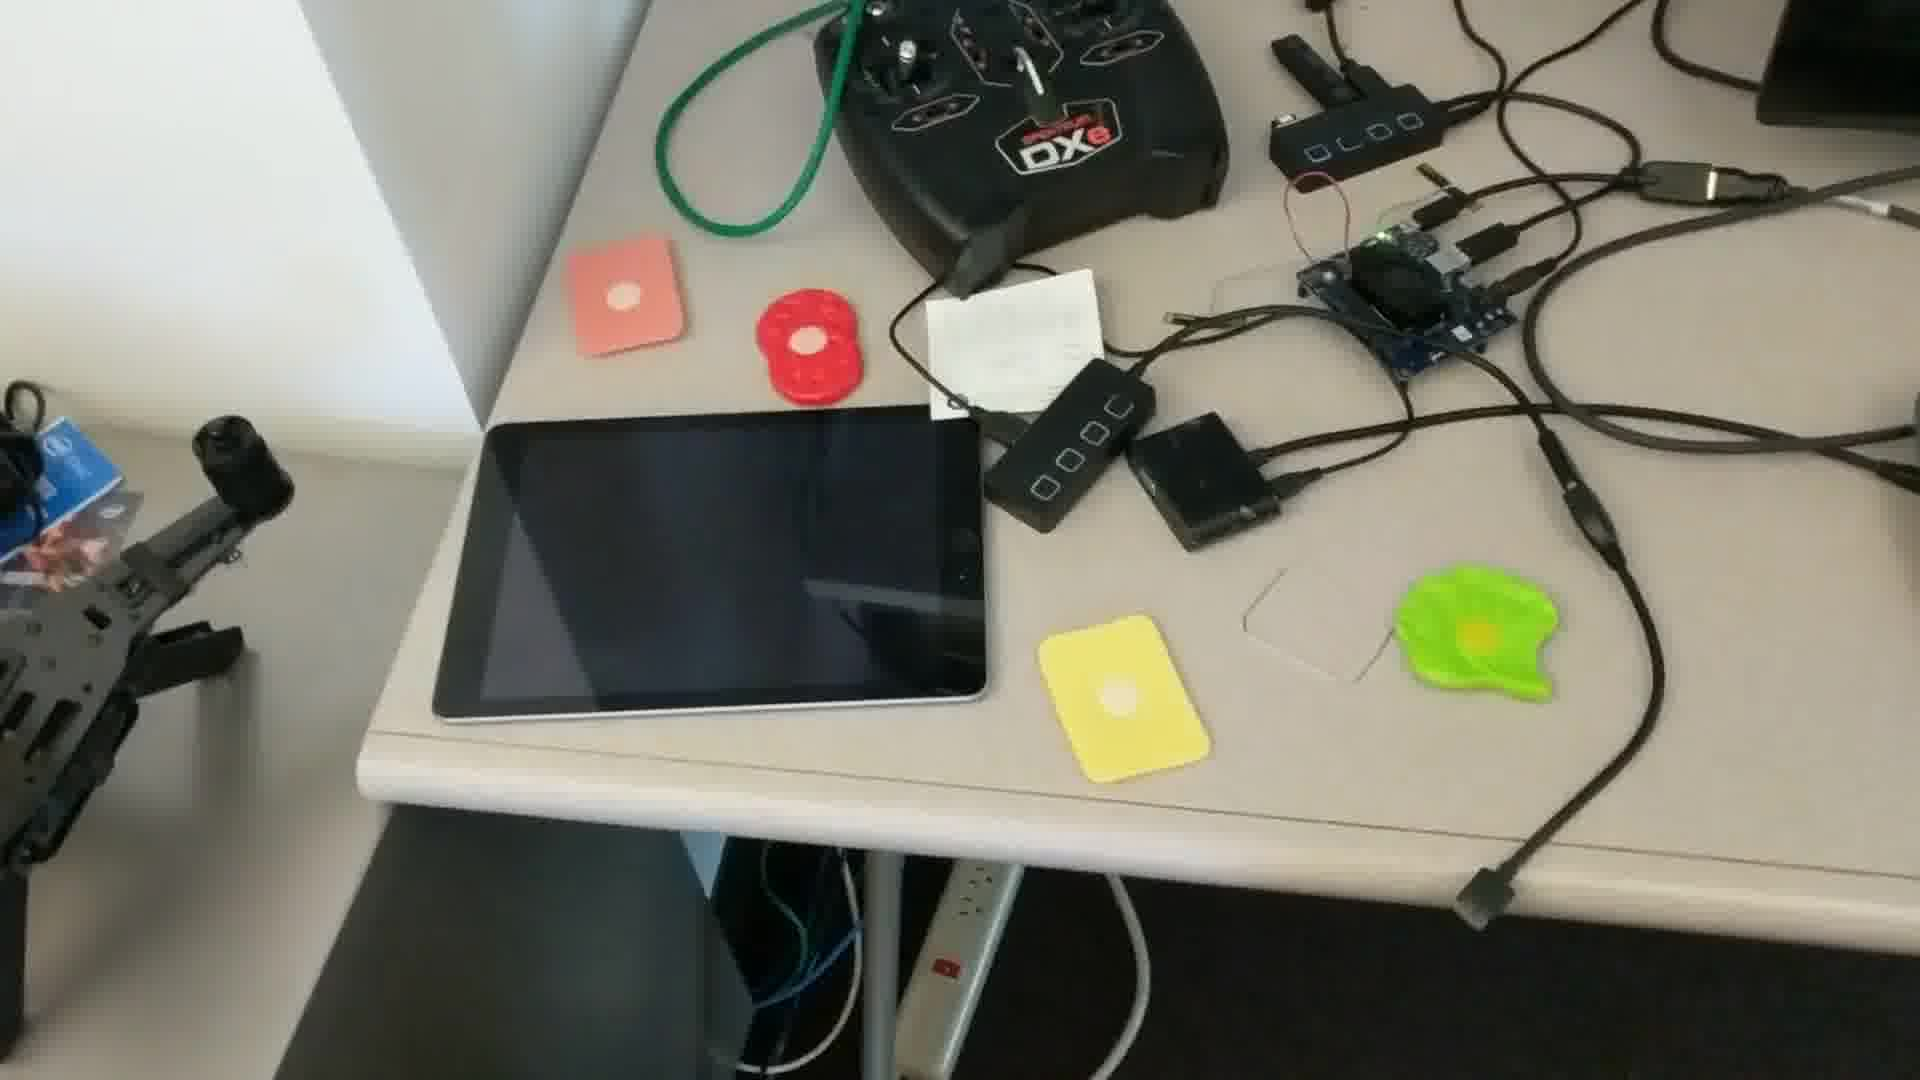
\includegraphics[width=\textwidth]{FIGS/sandwich-training-2.jpg}
  \end{minipage}
  \begin{minipage}[b]{0.32\textwidth}
    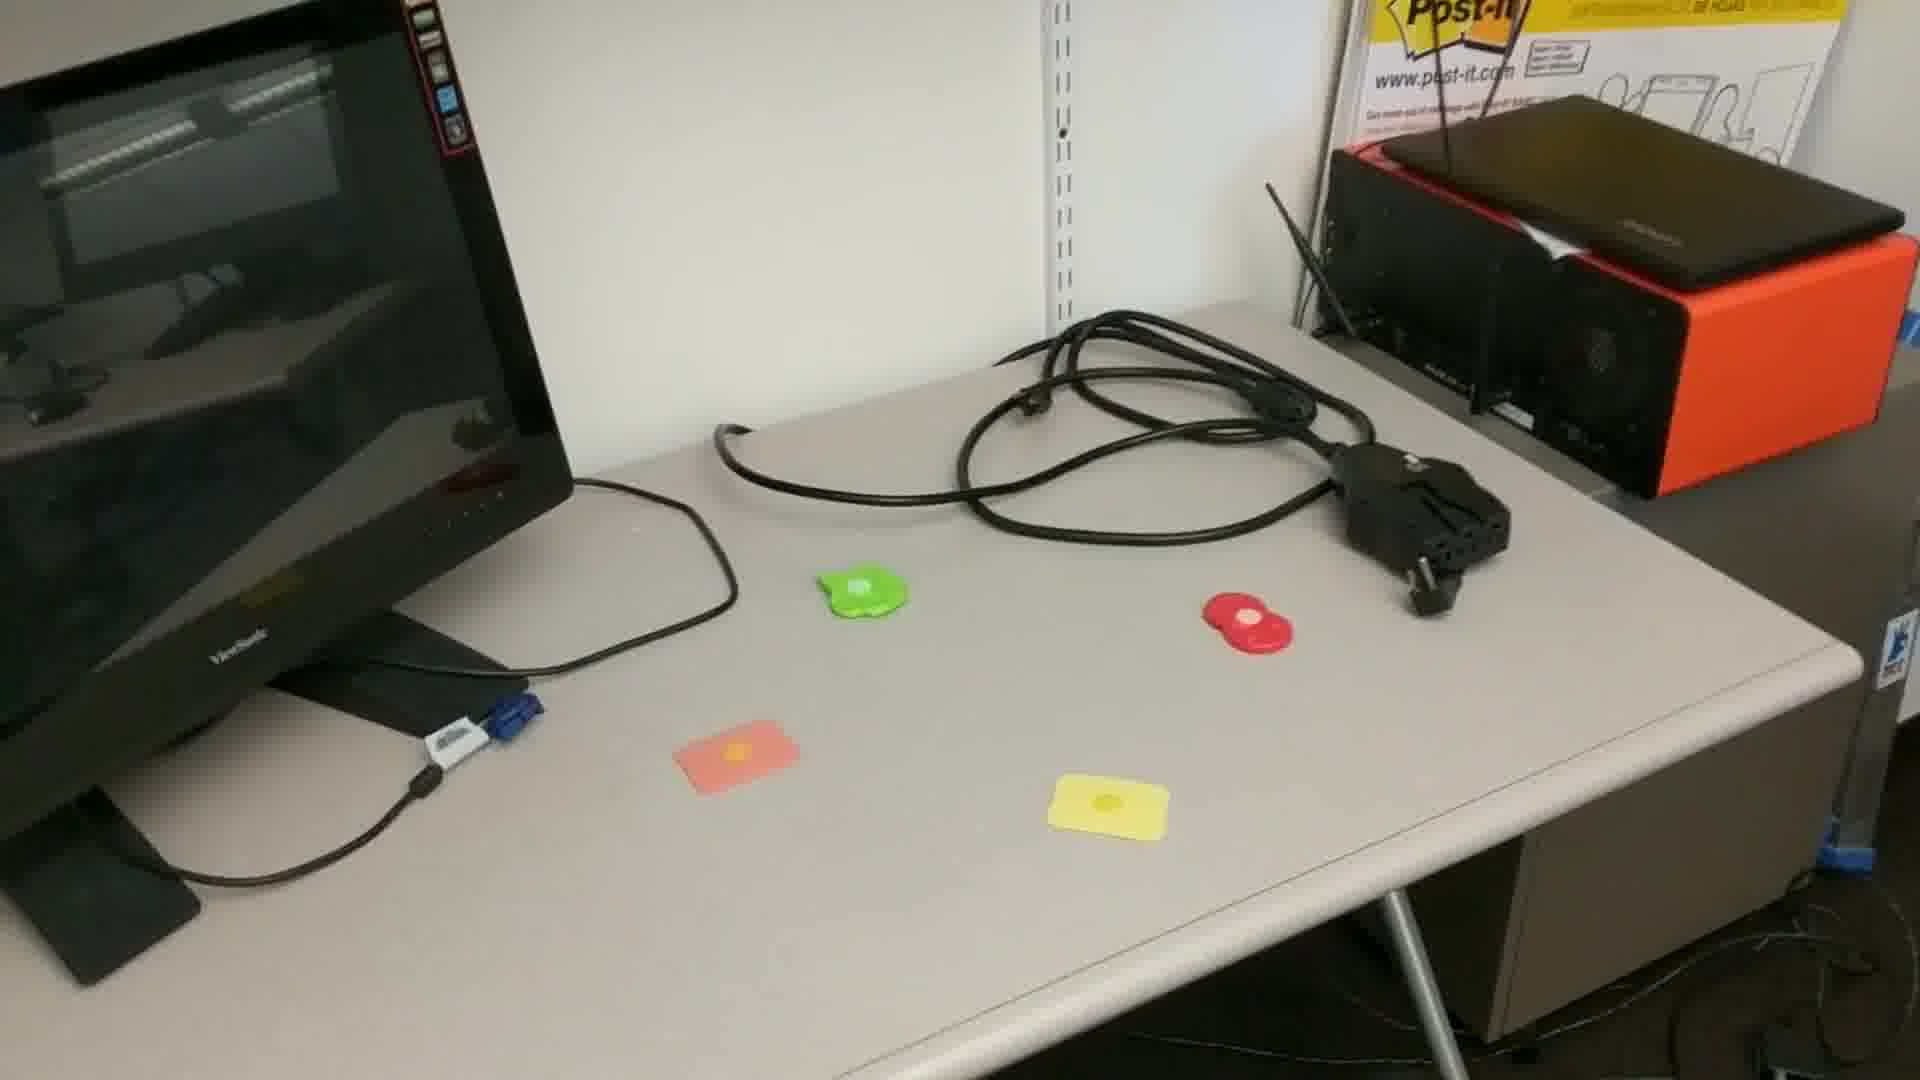
\includegraphics[width=\textwidth]{FIGS/sandwich-training-3.jpg}
  \end{minipage}
    \caption{TPOD Training Images Examples}
  \label{figs:tpod-example-training-images}
\end{figure}

Using TPOD to create object detectors is straight-forward. Developer first
captures videos of objects from various viewing angles and diverse backgrounds.
These videos can be captured on a mobile phone. At 30 frames per second, ten
mintues of video footage contain 18000 frames, which is already an acceptable
amount of training data for transfer learning. An larger amount of training data
typically helps increase the accuracy, although diminishing return also applies.
Moreover, it is preferred to collect training examples similar to the test
environment, as they present more suitable distribution for the model to learn.
Figure~\ref{figs:tpod-example-training-images} shows three example training
images for a toy cooking set. Note that the image background will be used as
negative examples to illustrate to the neural network about what an object does
not look like. Therefore, background better contains common objects in the test
environment that may cause wrong detections.


\begin{figure}[]
  \centering
    \fbox{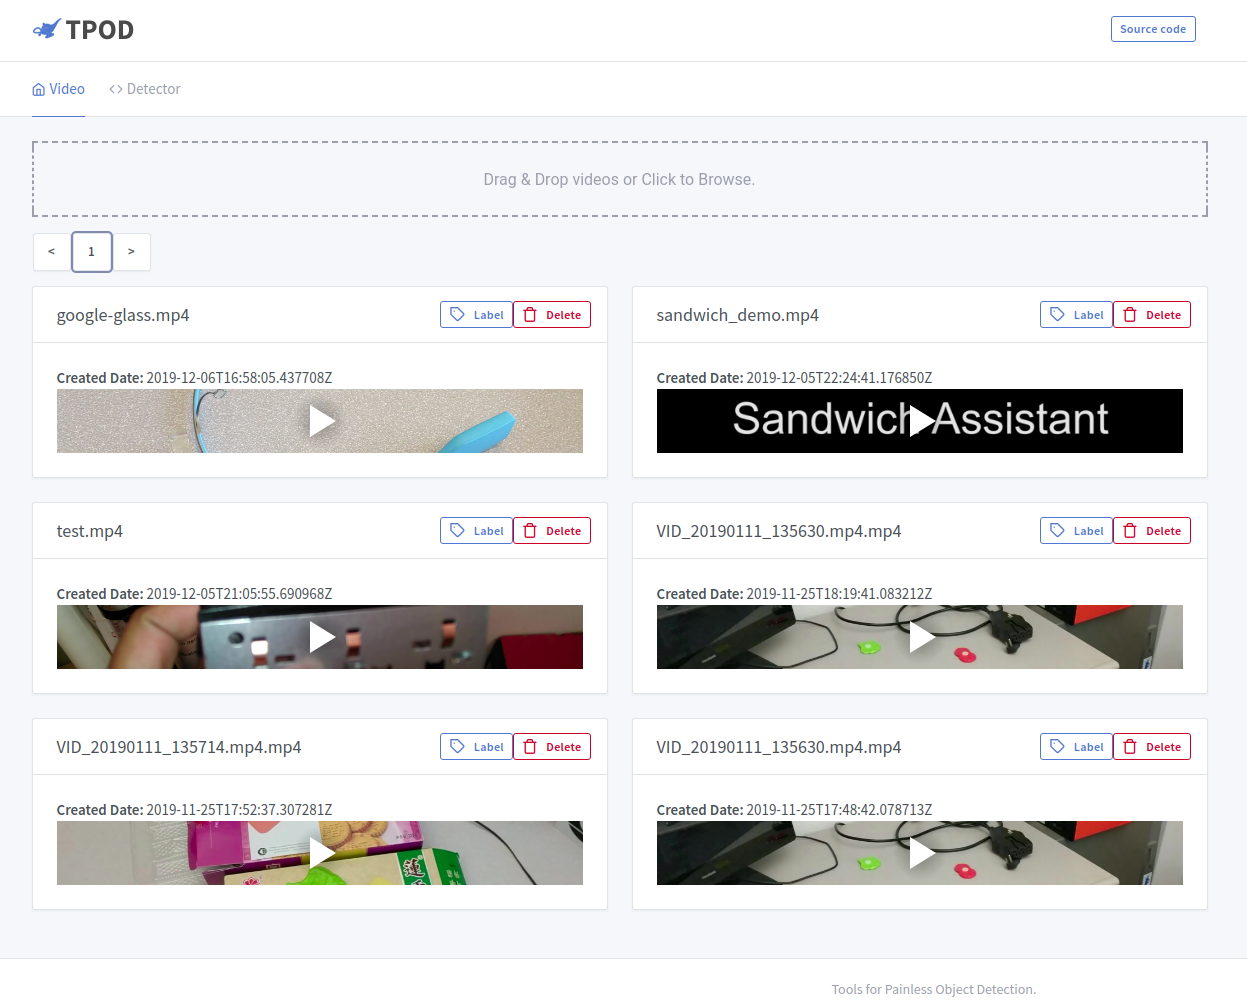
\includegraphics[width=\textwidth]{FIGS/tpod-video-gui}}
    \caption{TPOD Video Management GUI}
  \label{figs:tpod-video-gui}
\end{figure}

Next, developers upload the collected training videos to TPOD either directly
from the phone or from a computer. As shown in Figure~\ref{figs:tpod-video-gui},
TPOD helps user to store and organize training videos. TPOD helps users annotate
the training videos by integrating an external labeling tool into the GUI. Uers
annotate objects of interests by draw bounding boxes on the video frame. To help
facilitate the annotation process, TPOD leverages the fact that the frames are
part of a continuous video shot, and automatically generate bounding box in
subsequent frames using a correlation tracking
algorithm~\cite{danelljan2014accurate}. Therefore, users only need to label a
few key frames in a video with the rest of frames auto-populated with generated
labels. Of course, tracking is not perfect, and the bounding box may drift off
the object over time. In this case, the user can scroll forward or back in the
video, and adjust the bounding box to better match the object.  The adjustment
of bounding boxes reinitializes the tracking for subsequent frames. Overall,
this approach of labeling followed by tracking can reduce the number of frames
that the user needs to manually label by a factor of 10-20x.

\begin{figure}[]
  \centering
    \fbox{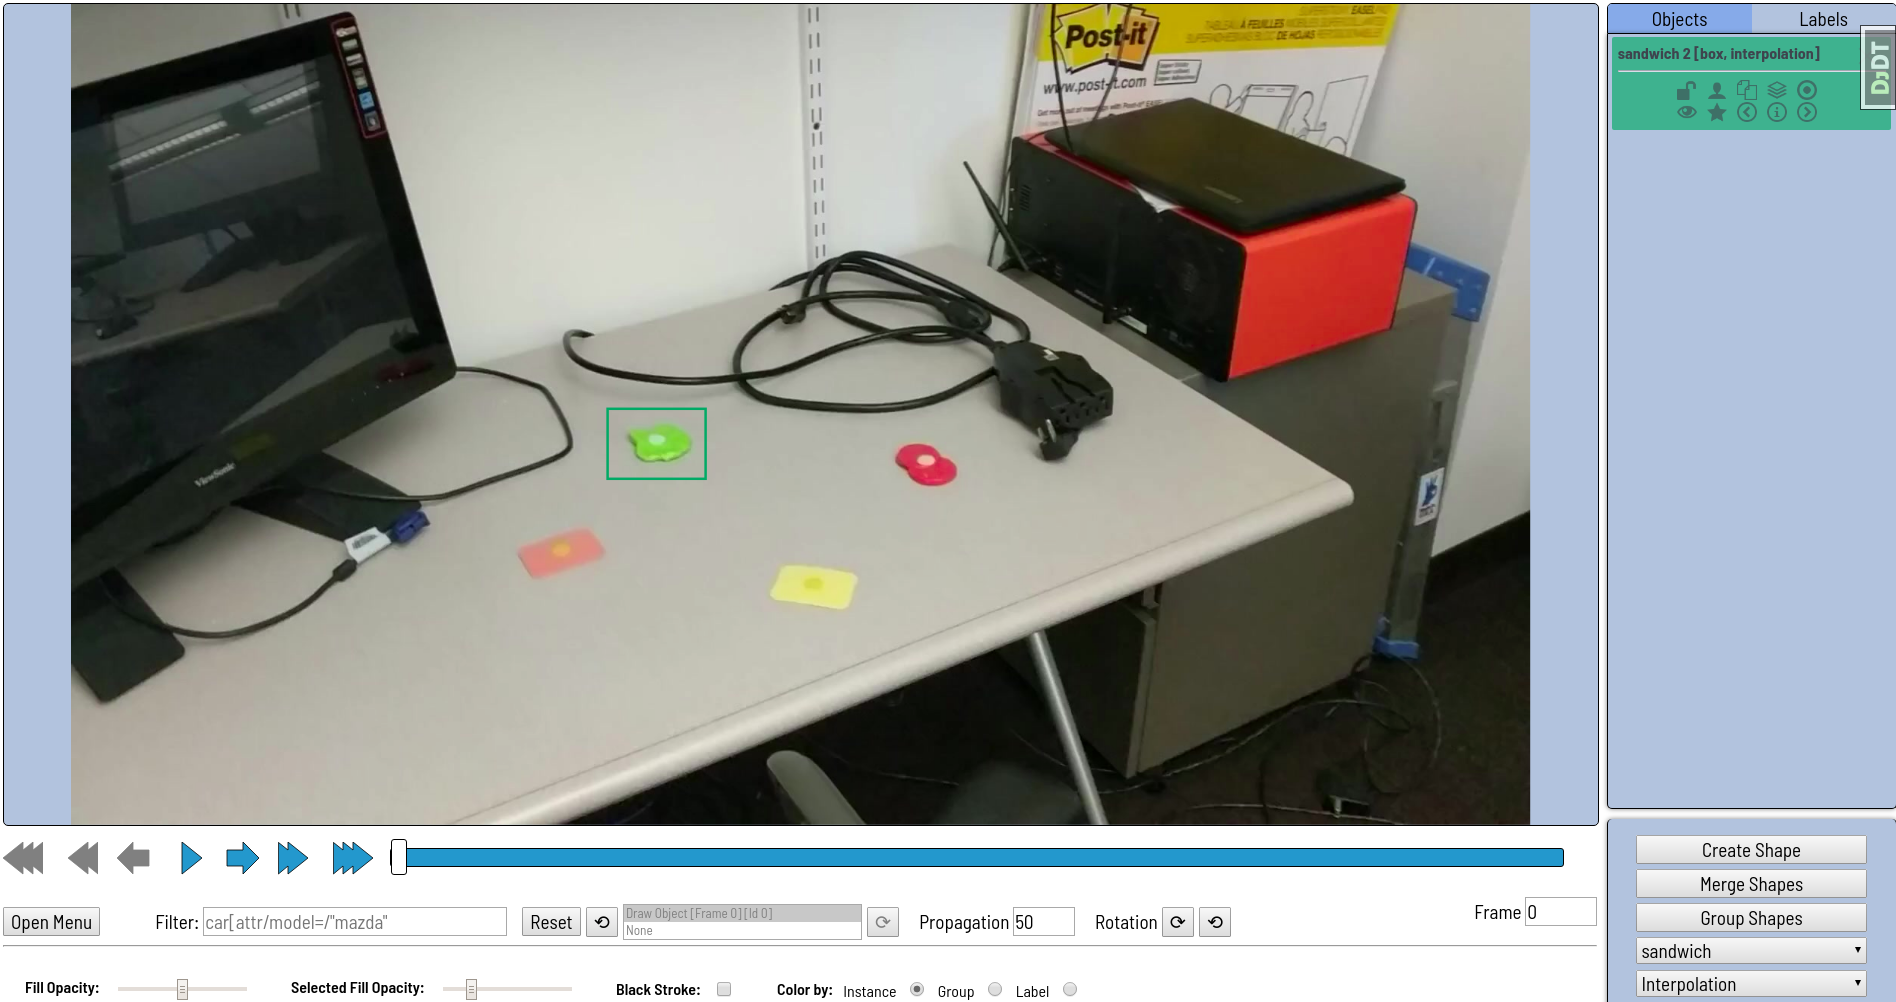
\includegraphics[width=\textwidth]{FIGS/tpod-label-gui}}
    \caption{TPOD Integration of an External Labeling Tool}
  \label{figs:tpod-label-gui}
\end{figure}

With videos annotated, users can move on to create dataset for training by
selecting videos to use. TPOD performs a data cleaning and augmentation pass to
prepare a high quality training set. Due to interframe correlations, adjacent
frames within the video may appear to be very similar or even identical. These
highly correlated frames violates the indepedent and identically distributed
assumption of training data for DNNs. TPOD eliminates these near duplicate
examples, as they would increase the model biases.  Optionally, data
augmentation can be employed. It adds synthetic images, created by cutting and
pasting the object of interests on varying backgrounds, at different scales and
rotations. Such augmentation has been shown to help produce more robust object
detectors~\cite{dwibedi2017cut}.

Then, by submitting a form on the web GUI, users can launch the DNN training
process with writing a single line of code. TPOD underneath automate the
transfer learning process of a DNN model using user specified dataset. TPOD
supports several state-of-the-art object detection network for transfer
learning, including FasterRCNN-ResNet~\cite{ren2015faster}~\cite{He2016} and
SSD-MobileNet~\cite{Liu2016}~\cite{Howard2017}. These different networks exhibit
different accuracy versus speed trade-off. While FasterRCNN-ResNet achieves
higher accuracies on standard datasets, its training and inference time are
significantly longer than SSD-MobileNet. Application developers should choose
the appropriate DNN network based on their accuracy and latency constraints.
Negative examples are mined from the video background; these are parts of the
frames not included in the object bounding boxes.  The training is started as a
batch process that uses a standard, scripted learning schedule, and generates
downloadable Tensorflow model in the end. The TPOD web interface provides
training monitoring and download links for the created model files. TPOD also
provides a container image that can directly serve the downloaded model files
for inference.

Overall, TPOD can greatly reduce both the labeling effort and in-depth machine
learning knowledge needed to effectively train and deploy a DNN-based detector.
The initial prototype of TPOD has been used by researchers and students to build
wearable cognitive assistance. For example, a group of master students in CMU
mobile and pervasive computing class successfully used TPOD to build an
assistant for using Automated External Defibrillator (AED) machines.

\subsection{TPOD Case Study for Cooking Application}

To quantify how much TPOD can help reduce laboring efforts in training object
detectors, we conduct a case study to train detectors for the Cooking cognitive
assistance~\cite{chen2018application}. We trained object detectors for 9
components of a toy sandwich, including bread, ham, lettuce, cucumber, cheese,
half sandwich, ham wrong state, tomato, and full sandwich. We collected 53 short
training videos, annotated all videos, and trained object detectors all with
TPOD.

In total, we collected 21218 frames with the videos. When using TPOD's labeling,
we only manually labeled 91 frames. The rest of frames are automatically labeled
by TPOD's tracking component. The total labeling session lasted 80 minutes. The
total number of frames used for training is 21013, because of data set
optimization. We fine-tuned from a FasterRCNN-VGG network. The finetuning
process took 54 minutes to finish on a NVIDIA K40c GPU.


\subsection{TPOD Architecture}

\begin{figure}[]
  \hspace{-.1in}
    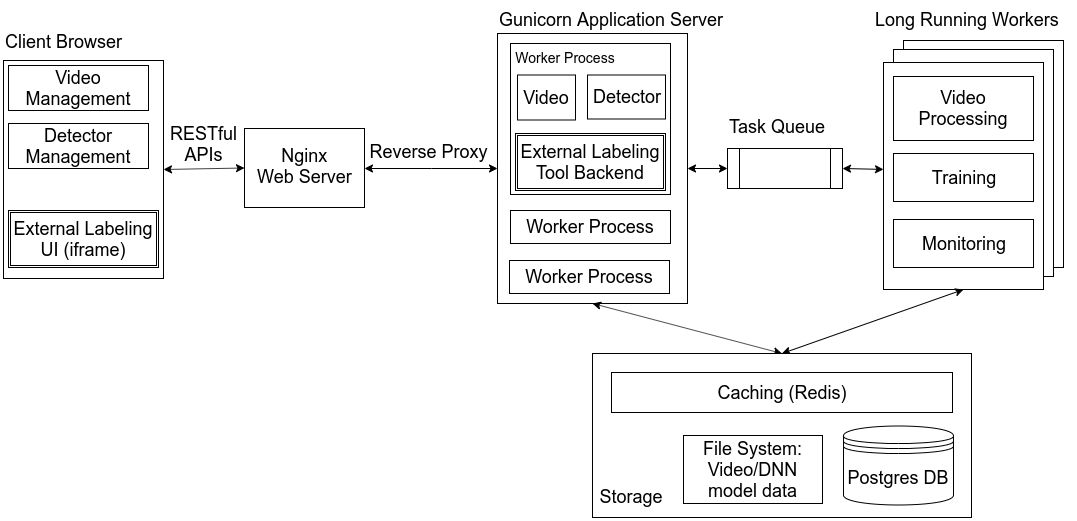
\includegraphics[width=1.1\textwidth]{FIGS/tpod-arch}
    \caption{TPOD Architecture}
  \label{figs:tpod-arch}
\end{figure}

TPOD adopts a Model-View-Controller (MVC) design for web
applications~\cite{krasner1988description}. Figure~\ref{figs:tpod-arch} shows
TPOD architecture. TPOD frontend handles UI logic and is built using React, a
declarative, efficient, and flexible JavaScript library for creating user
interface~\cite{staff2016react}. React enable TPOD frontend code to be modular
and reusable. The frontend has three major components: video management,
detector management, and an external labeling tool. TPOD integrate the labeling
tool CVAT~\cite{cvat2019} into its frontend through embedding via an iframe. The
embedding of an labeling tool directly into the GUI unifies the workflow to
eliminate users' need to set up and use another piece of software. TPOD frontend
communicates with the backend using a set of RESTful
apis~\cite{richardson2008restful}, centered around \textit{Video} and
\textit{Detector} resources. 

TPOD backend is developed using the Django web
framework~\cite{holovaty2009definitive} and served with Nginx web
server~\cite{nedelcu2010nginx} and Gunicorn application
server~\cite{gunicorn2017http}. The backend implements the RESTful apis to
create, read, update, and delete \textit{Video} and \textit{Detector} resources.
It also interface with the external labeling tool CVAT's backend to read and
write annotations. Long running background jobs, such as DNN model training and
video extraction is processed asynchronously using a task queue and
long running worker processes. Metadata about videos and DNN models are stored
in a relational database while large binary files, such as video files and
trained DNN model weights are stored in the file system. An in-memory caching
layer on top of the file system and database is created using key-value store
Redis. The entire application is containerized and can be deployed easily onto
bare-metal or virtualized environment.

One key design choice of TPOD is to be extensible for new DNN architectures.
TPOD provide a standard interface, shown in
Figure~\ref{figs:tpod-provider-interface} to add new DNNs implementation for
transfer learning. TPOD refers to these DNN implementations as DNN
\textit{Providers}. Providers do no need to know anything else about TPOD and
only need to implement the Provider interface to be integrated and used. The
built-in \textit{Provider} is Tensorflow's object detection API, which supports
transfer learning for a wide set of object detectors~\cite{tfod2019}. 


\begin{algorithm} 
% \addcontentsline{TPOD Provider Interface}{algorithm}{TPOD Provider Interface}
\SetAlgoLined
 property \textbf{training\_configurations}: user customizable hyperparameters\;
 \textbf{init(dnn\_type, training\_set, output\_directory)}: initialization\;
 \textbf{train(training\_configurations)}: launch training\;
 \textbf{export()}: export trained models\;
 \textbf{visualization()}: monitor training process\;
\caption{TPOD Provider Interface}
\label{figs:tpod-provider-interface}
\end{algorithm}
\section{Finite State Machine (FSM) Authoring Tools}
\label{sec: app-dev-fsm}

In addition to creating DNN-based object detectors, developers need to write
custom logic to implement the WCA task model running on the cloudlet. In this
section, we introduce a FSM authoring tool that provides libraries and GUI to
enable fast implementation to allow for quick development iteration.

As discussed in Section~\ref{sec: app-dev-fsm-representation}, WCA cloudlet
logic can be represented as a finite state machine. The FSM representation
allows us to impose structure and provide tools for task model implementation.
Our FSM authoring tool consists of a web GUI that allows users to visualize and
edit a WCA FSM within a browser, a python library that supports the creation and
execution of a FSM, and a binary file format that efficiently stores the FSM.

\subsection{FSM Editor}

\begin{figure}
    \centering
    \fbox{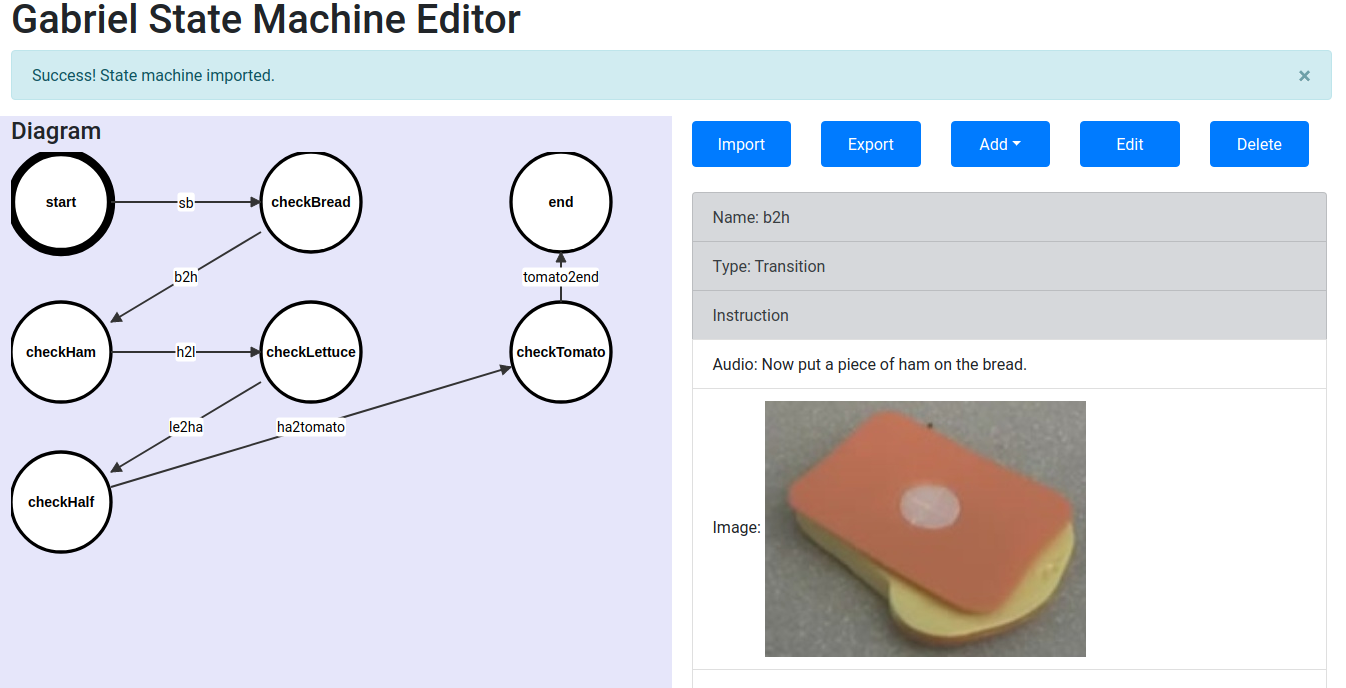
\includegraphics[trim={0 0 0 0},width=\linewidth]{FIGS/fsm-web-gui}}
	\caption{FSM Web GUI}
    \label{figs:fsm-web-gui}
\end{figure}

Figure~\ref{figs:fsm-web-gui} shows our FSM Web Editor. Users can create a WCA
FSM from the GUI by editing states and transitions. State processors, e.g. the
computer vision processing logic to run in a given state, can be specified by a
container url. User guidance can be added through adding text, video urls or by
uploading images. The Web GUI also supports import and export functionalities to
interface with other WCA tools. The exported FSM is in a custom binary format
and can be executed by FSM python library.

The GUI is implemented as a pure browser-based user interface, using
React~\cite{staff2016react}. No web backend is needed. This makes the GUI easy
to set up and deploy. User only needs to open an HTML file in a browser to 
use the tool.

\subsection{FSM Python Library}

Another way to programmatically create a FSM is through the FSM Python library.
The library provides python APIs to create and modify FSMs. The python APIs
provides additional interfaces to add custom computer vision processing as
functions and ad hoc transition predicates for customization. 

In addition, the Python library provides a state machine executor that takes a
WCA FSM (e.g. made with the Web GUI) and launches a WCA program using the
Gabriel platform. The program is then ready to be connected by Gabriel Android
Client. The WCA program follows the logic defined in the state machine. A
Jupyter Notebook~\cite{kluyver2016jupyter} is also provided to make it possible to launch the program from
a browser. This library has been made available on The Python Package Index for
easy installation.

\subsection{FSM Binary Format}

We define a custom FSM binary format for WCAs that can be read and wrote using
multiple programming languages. We use serialization library Protocol Buffers to
generate language-specific stub code. Figure~\ref{figs:fsm-binary-format} shows
a summary of the serialization format.


\begin{figure}
\small
\begin{lstlisting}
// represents the trigger condition
message TransitionPredicate {
  string name = 1;
  string callable_name = 2; 
  map<string, bytes> callable_kwargs = 3; // arguments
  string callable_args = 4; // arguments
}

message Instruction {
  string name = 1;
  string audio = 2; // audio in text format.
  bytes image = 3;
  bytes video = 4;
}

message Transition {
  string name = 1;
  // function name of the trigger condition
  repeated TransitionPredicate predicates = 2;
  Instruction instruction = 3;
  string next_state = 4;
}

// represent feature extraction modules
message Processor {
  // input are images
  // outputs are key/value pairs that represents application state
  string name = 1;
  string callable_name = 2; 
  map<string, bytes> callable_kwargs = 3; // arguments
  string callable_args = 4; // arguments
}

message State {
  string name = 1;
  repeated Processor processors = 2; // extract features
  repeated Transition transitions = 3;
}

message StateMachine {
  string name = 1;
  repeated State states = 2; // all states
  map<string, bytes> assets = 3; // shared assets
  string start_state = 4;
}
\end{lstlisting}
\caption{FSM Binary Format}
\label{figs:fsm-binary-format}
\end{figure}

% We observed that the
% implementation of a cognitive assistant mainly consists of components to
% identify user states using computer vision models, specify instructions to users
% based on the current state, and keep track of progress on the task. We created a
% a workflow modeling tool, SME, which can transform the process of completing a
% task into a specific model, substantially reducing the expert modeling effort
% required. By using a framework to reason about step-by-step application, along
% with workflow information from WE and object recognition models from TPOD, SME
% also automatically generates a Gabriel executable application based on the
% modeled workflow.

% The applications SME generates are defined by a set of steps. Each state
% corresponds to the subset of steps that a user has completed. We use a FSM to
% keep track of the current state of a task and the future states that we should
% transition to when a user takes a certain action. Transitions among states are
% triggered by visual changes resulting from user actions. For example, the user
% might put a piece of ham on top of a piece of bread. In addition, each state has
% its own processing functions, which convert the current visual state into
% information that the application can understand. We provide a list of
% pre-defined processing functions, such as object detection DNNs. Task experts
% also have the flexibility to add custom processing functions when needed.
% Figure~\ref{fig:sme} shows a sample workflow as a finite state machine. Once the
% task expert finalizes a FSM, SME automatically compile the FSM to generate an
% executable application.

\section{Chapter Summary and Discussion}

Wearable cognitive assistance is difficult to develop due to the high barrier of
entry and the lack of development methodology and tools. In this chapter, we
present a unifying development methodology, centered around object detection and
finite state machine representation to systematize the development process.
Based on this methodology, we build a suite of development tools that helps
object detector creation and speed up task model implementation. 

% Previous
% experience with these tools, we have shown the productivity improvement can be 10x-20x for application
% developers.